\chapter{Resultados e Análise Computacional} \label{ch:resultados}

\section{Instâncias e Ambiente de Testes}

Os experimentos computacionais foram realizados utilizando um conjunto de 42 instâncias de teste geradas sinteticamente, representando diferentes cenários do Problema da Distribuição de Disciplinas (DPD). As instâncias variam em tamanho e complexidade, com número de disciplinas entre 62 e 214, número de professores entre 22 e 69, e diferentes configurações de áreas de conhecimento e preferências.

Para cada experimento, foram selecionadas aleatoriamente 10 instâncias dentre as 42 disponíveis, garantindo representatividade estatística enquanto mantém o tempo total de experimentação viável. Cada instância foi escolhida de maneira aleatória dentro do conjunto de arquivos de entrada. As mesmas instâncias foram utilizadas em todas as configurações testadas de um mesmo parâmetro, assegurando comparabilidade direta dos resultados.

Todas as execuções foram realizadas com limite de tempo global de 400 segundos por instância. O solver utilizado foi o SCIP 7.0, integrado com as heurísticas LNS e GRASP desenvolvidas neste trabalho. 

A análise dos parâmetros da heurística LNS foi conduzida de forma incremental: primeiro determinou-se a melhor taxa de destruição, em seguida o melhor sentido de ordenação, e finalmente o melhor limite de tempo para o sub-MIP. Esta abordagem sistemática permite isolar o impacto de cada parâmetro e identificar a configuração ótima.

\section{Análise Interna das Configurações da LNS}

\subsection{Impacto da Taxa de Destruição (10\%, 25\%, 50\% e 75\%)}

A primeira análise experimental investigou o impacto da taxa de destruição (\texttt{lns\_perc}) na qualidade das soluções e no desempenho computacional. Foram testadas quatro configurações: 10\%, 25\%, 50\% e 75\% de destruição, mantendo fixos o tempo máximo do LNS (30s por chamada), a ordenação (crescente) e o tempo total de execução (400s).

\textbf{Resultados de Tempo de Execução:} A Tabela~\ref{tab:lns_cand_tempo} apresenta o tempo total de execução para 10 instâncias selecionadas. A configuração de relaxação (sem LNS) obteve o melhor desempenho médio, com 19,49 segundos, contra 25,39 segundos da melhor configuração LNS. Entretanto, sete das dez instâncias foram resolvidas de forma ótima (tempo reduzido), enquanto três instâncias (input7, input15 e input22) atingiram o limite de tempo. Este resultado indica que o tempo adicional investido pelo LNS não se traduz necessariamente em melhoria para instâncias fáceis, mas pode ser crucial para instâncias difíceis.

% ============================================
% TABELAS - RESULTADOS DOS EXPERIMENTOS LNS
% ============================================

% Pacotes necessários: booktabs, multirow, array

% ============================================
% TABELA 1: Impacto da Taxa de Destruição - Tempo
% ============================================
\begin{table}[htbp]
\centering
\caption{Tempo de execução (segundos) para diferentes taxas de destruição do LNS. Configuração: ordenação crescente, tempo LNS = 30s, limite global = 400s.}
\label{tab:lns_cand_tempo}
\small
\begin{tabular}{@{}lrrrrrrrr@{}}
\toprule
\textbf{Instância} & \textbf{Disciplinas} & \textbf{Profs} & \textbf{Relax.} & \textbf{10\%} & \textbf{25\%} & \textbf{50\%} & \textbf{75\%} & \textbf{Melhor} \\
\midrule
input2  & 79  & 24 & 4,04    & 17,07  & 17,66  & 16,98  & 17,04  & Relax. \\
input5  & 84  & 29 & 113,03  & 145,27 & 145,04 & 145,71 & 143,63 & Relax. \\
input6  & 113 & 31 & 1,07    & 2,47   & 2,40   & 2,33   & 2,22   & Relax. \\
input7  & 99  & 28 & 400,02  & 400,02 & 400,02 & 400,02 & 400,02 & Empate \\
input9  & 133 & 41 & 17,06   & 72,52  & 72,33  & 72,57  & 73,48  & Relax. \\
input13 & 125 & 39 & 29,13   & 60,21  & 59,56  & 59,04  & 59,43  & Relax. \\
input19 & 114 & 39 & 2,11    & 1,39   & 1,44   & 1,42   & 1,47   & LNS 10\% \\
input20 & 113 & 40 & 0,95    & 4,69   & 4,56   & 4,59   & 5,02   & Relax. \\
input26 & 185 & 60 & 33,73   & 25,50  & 24,67  & 24,81  & 24,38  & LNS 75\% \\
input34 & 137 & 42 & 21,92   & 26,68  & 26,08  & 26,38  & 26,41  & Relax. \\
\midrule
\textbf{Média}  & 114 & 39 & 19,49 & 25,38 & 25,38 & 25,59 & 25,39 & Relax. \\
\textbf{Total}  & 1.296 & 412 & \textbf{623,05} & 755,82 & 753,76 & 753,84 & 753,10 & \textbf{Relax.} \\
\bottomrule
\end{tabular}
\end{table}

% ============================================
% TABELA 2: Impacto da Taxa de Destruição - Nodes Left
% ============================================
\begin{table}[htbp]
\centering
\caption{Número de nós restantes na árvore de Branch-and-Bound para diferentes taxas de destruição. Valores menores indicam maior progresso em direção à otimalidade.}
\label{tab:lns_cand_nodes}
\small
\begin{tabular}{@{}lrrrrrrrr@{}}
\toprule
\textbf{Instância} & \textbf{Disciplinas} & \textbf{Profs} & \textbf{Relax.} & \textbf{10\%} & \textbf{25\%} & \textbf{50\%} & \textbf{75\%} & \textbf{Melhor} \\
\midrule
input2  & 79  & 24 & 0      & 0      & 0      & 0      & 0      & -- \\
input5  & 84  & 29 & 0      & 0      & 0      & 0      & 0      & -- \\
input6  & 113 & 31 & 0      & 0      & 0      & 0      & 0      & -- \\
input7  & 99  & 28 & 66.230 & 62.628 & 60.540 & 61.056 & \textbf{58.921} & \textbf{75\%} \\
input9  & 133 & 41 & 0      & 0      & 0      & 0      & 0      & -- \\
input13 & 125 & 39 & 0      & 0      & 0      & 0      & 0      & -- \\
input19 & 114 & 39 & 0      & 0      & 0      & 0      & 0      & -- \\
input20 & 113 & 40 & 0      & 0      & 0      & 0      & 0      & -- \\
input26 & 185 & 60 & 0      & 0      & 0      & 0      & 0      & -- \\
input34 & 137 & 42 & 0      & 0      & 0      & 0      & 0      & -- \\
\midrule
\textbf{Média}  & 114 & 39 & 6.623 & 6.263 & 6.054 & 6.106 & 5.892 & LNS 75\% \\
\textbf{Total}  & 1.296 & 412 & 66.230 & 62.628 & 60.540 & 61.056 & \textbf{58.921} & \textbf{LNS 75\%} \\
\bottomrule
\end{tabular}
\end{table}

% ============================================
% TABELA 3: Impacto da Ordenação - Tempo
% ============================================
\begin{table}[htbp]
\centering
\caption{Tempo de execução (segundos) comparando ordenação crescente e decrescente. Configuração: 75\% de destruição, tempo LNS = 30s, limite global = 400s.}
\label{tab:lns_order_tempo}
\small
\begin{tabular}{@{}lrrrrrr@{}}
\toprule
\textbf{Instância} & \textbf{Disciplinas} & \textbf{Profs} & \textbf{Relax.} & \textbf{Crescente} & \textbf{Decrescente} & \textbf{Melhor} \\
\midrule
input4  & 123 & 46 & 400,05 & 400,04 & 400,05 & Crescente \\
input5  & 214 & 69 & 114,18 & 140,64 & 141,47 & Crescente \\
input12 & 115 & 37 & 5,79   & 25,70  & 25,84  & Crescente \\
input15 & 94  & 30 & 400,03 & 400,02 & 400,02 & Decrescente \\
input16 & 89  & 28 & 3,07   & 0,72   & 0,72   & Decrescente \\
input17 & 108 & 38 & 400,04 & 400,04 & 400,03 & Decrescente \\
input20 & 104 & 37 & 0,90   & 4,40   & 4,32   & Decrescente \\
input33 & 104 & 36 & 400,03 & 400,03 & 400,03 & Decrescente \\
input37 & 152 & 53 & 68,00  & 31,61  & 31,62  & Crescente \\
input38 & 62  & 22 & 0,16   & 0,28   & 0,28   & Decrescente \\
\midrule
\textbf{Média}  & 106 & 37 & 91,09 & 180,31 & 180,38 & Crescente \\
\textbf{Total}  & 1.271 & 433 & \textbf{1.792,24} & 1.803,48 & 1.804,48 & \textbf{Relax.} \\
\bottomrule
\end{tabular}
\end{table}

% ============================================
% TABELA 4: Impacto da Ordenação - Nodes Left
% ============================================
\begin{table}[htbp]
\centering
\caption{Número de nós restantes comparando ordenação crescente e decrescente.}
\label{tab:lns_order_nodes}
\small
\begin{tabular}{@{}lrrrrrr@{}}
\toprule
\textbf{Instância} & \textbf{Disciplinas} & \textbf{Profs} & \textbf{Relax.} & \textbf{Crescente} & \textbf{Decrescente} & \textbf{Melhor} \\
\midrule
input4  & 123 & 46 & 19.797 & 19.541 & 19.507 & Decrescente \\
input5  & 214 & 69 & 0      & 0      & 0      & -- \\
input12 & 115 & 37 & 0      & 0      & 0      & -- \\
input15 & 94  & 30 & 64.711 & \textbf{61.546} & 62.452 & \textbf{Crescente} \\
input16 & 89  & 28 & 0      & 0      & 0      & -- \\
input17 & 108 & 38 & 4.673  & 4.667  & 4.652  & Decrescente \\
input20 & 104 & 37 & 0      & 0      & 0      & -- \\
input33 & 104 & 36 & 50.279 & \textbf{46.243} & 47.063 & \textbf{Crescente} \\
input37 & 152 & 53 & 0      & 0      & 0      & -- \\
input38 & 62  & 22 & 0      & 0      & 0      & -- \\
\midrule
\textbf{Média}  & 106 & 37 & 13.946 & 13.200 & 13.367 & Crescente \\
\textbf{Total}  & 1.271 & 433 & 139.460 & \textbf{131.997} & 133.674 & \textbf{Crescente} \\
\bottomrule
\end{tabular}
\end{table}

% ============================================
% TABELA 5: Impacto do Tempo Máximo LNS - Tempo
% ============================================
\begin{table}[htbp]
\centering
\caption{Tempo de execução (segundos) para diferentes limites de tempo do sub-MIP. Configuração: 75\% de destruição, ordenação crescente, limite global = 400s.}
\label{tab:lns_time_tempo}
\small
\begin{tabular}{@{}lrrrrrrrrr@{}}
\toprule
\textbf{Inst.} & \textbf{Disc.} & \textbf{Prof.} & \textbf{Relax.} & \textbf{10s} & \textbf{50s} & \textbf{100s} & \textbf{200s} & \textbf{Melhor} \\
\midrule
input6  & 79  & 24 & 1,19   & 2,40   & 2,14   & 2,15   & \textbf{2,14}   & \textbf{200s} \\
input14 & 99  & 28 & 14,21  & 22,31  & 68,47  & 118,44 & 168,12 & Relax. \\
input15 & 94  & 30 & 400,03 & 400,02 & 400,02 & \textbf{76,31} & 77,09 & \textbf{100s} \\
input21 & 104 & 31 & 6,98   & \textbf{3,02}   & 3,04   & 3,05   & 3,10   & \textbf{10s} \\
input22 & 133 & 41 & 400,05 & 400,04 & 400,04 & 400,04 & 400,04 & 10s \\
input23 & 118 & 35 & 1,55   & \textbf{11,41} & 12,80  & 12,66  & 12,50  & \textbf{10s} \\
input27 & 125 & 39 & 4,93   & 7,45   & 7,34   & 7,33   & \textbf{7,31}   & \textbf{200s} \\
input29 & 103 & 39 & 400,03 & 400,03 & 19,42  & 19,40  & \textbf{19,39}  & \textbf{200s} \\
input33 & 104 & 36 & 400,03 & 400,03 & 400,03 & 400,03 & 400,03 & 200s \\
input38 & 62  & 22 & 0,16   & 0,28   & 0,28   & \textbf{0,28}   & 0,28   & \textbf{100s} \\
\midrule
\textbf{Média} & 104 & 33 & 162,92 & 164,77 & 162,11 & 160,27 & \textbf{159,46} & \textbf{200s} \\
\textbf{Total} & 1.125 & 358 & 1.629,16 & 1.647,01 & 1.313,60 & \textbf{1.039,68} & 1.090,00 & \textbf{100s} \\
\bottomrule
\end{tabular}
\end{table}

% ============================================
% TABELA 6: Impacto do Tempo Máximo LNS - Nodes Left
% ============================================
\begin{table}[htbp]
\centering
\caption{Número de nós restantes para diferentes limites de tempo do sub-MIP.}
\label{tab:lns_time_nodes}
\small
\begin{tabular}{@{}lrrrrrrrrr@{}}
\toprule
\textbf{Inst.} & \textbf{Disc.} & \textbf{Prof.} & \textbf{Relax.} & \textbf{10s} & \textbf{50s} & \textbf{100s} & \textbf{200s} & \textbf{Melhor} \\
\midrule
input6  & 79  & 24 & 0      & 0      & 0      & 0      & 0      & -- \\
input14 & 99  & 28 & 0      & 0      & 0      & 0      & 0      & -- \\
input15 & 94  & 30 & 54.355 & 63.056 & 59.819 & \textbf{0} & \textbf{0} & \textbf{100s} \\
input21 & 104 & 31 & 0      & 0      & 0      & 0      & 0      & -- \\
input22 & 133 & 41 & 21.528 & 29.161 & \textbf{25.100} & 50.411 & 33.000 & \textbf{50s} \\
input23 & 118 & 35 & 0      & 0      & 0      & 0      & 0      & -- \\
input27 & 125 & 39 & 0      & 0      & 0      & 0      & 0      & -- \\
input29 & 103 & 39 & 12.643 & 4.347  & \textbf{0} & \textbf{0} & \textbf{0} & \textbf{50s} \\
input33 & 104 & 36 & 47.460 & 48.110 & 45.505 & 1.524  & \textbf{539} & \textbf{200s} \\
input38 & 62  & 22 & 0      & 0      & 0      & 0      & 0      & -- \\
\midrule
\textbf{Média} & 104 & 33 & 13.599 & 14.467 & 13.042 & 5.194 & \textbf{3.354} & \textbf{200s} \\
\textbf{Total} & 1.125 & 358 & 135.986 & 144.674 & 130.424 & 51.935 & \textbf{33.539} & \textbf{200s} \\
\bottomrule
\end{tabular}
\end{table}

% ============================================
% TABELA 7: Impacto da Taxa de Destruição - GAP
% ============================================
\begin{table}[htbp]
\centering
\caption{Gap de otimalidade (\%) para diferentes taxas de destruição. Gap igual a zero indica solução ótima.}
\label{tab:lns_cand_gap}
\small
\begin{tabular}{@{}lrrrrrrrr@{}}
\toprule
\textbf{Instância} & \textbf{Disciplinas} & \textbf{Profs} & \textbf{Relax.} & \textbf{10\%} & \textbf{25\%} & \textbf{50\%} & \textbf{75\%} & \textbf{Melhor} \\
\midrule
input2  & 79  & 24 & 0,00 & 0,00 & 0,00 & 0,00 & 0,00 & Empate \\
input5  & 84  & 29 & 0,00 & 0,00 & 0,00 & 0,00 & 0,00 & Empate \\
input6  & 113 & 31 & 0,00 & 0,00 & 0,00 & 0,00 & 0,00 & Empate \\
input7  & 99  & 28 & 0,60 & 0,60 & 0,60 & 0,60 & 0,60 & Empate \\
input9  & 133 & 41 & 0,00 & 0,00 & 0,00 & 0,00 & 0,00 & Empate \\
input13 & 125 & 39 & 0,00 & 0,00 & 0,00 & 0,00 & 0,00 & Empate \\
input19 & 114 & 39 & 0,00 & 0,00 & 0,00 & 0,00 & 0,00 & Empate \\
input20 & 113 & 40 & 0,00 & 0,00 & 0,00 & 0,00 & 0,00 & Empate \\
input26 & 185 & 60 & 0,00 & 0,00 & 0,00 & 0,00 & 0,00 & Empate \\
input34 & 137 & 42 & 0,00 & 0,00 & 0,00 & 0,00 & 0,00 & Empate \\
\midrule
\textbf{Média}  & 114 & 39 & 0,06 & 0,06 & 0,06 & 0,06 & 0,06 & Empate \\
\textbf{Total}  & 1.296 & 412 & 0,60 & 0,60 & 0,60 & 0,60 & 0,60 & \textbf{Empate} \\
\bottomrule
\end{tabular}
\end{table}

% ============================================
% TABELA 8: Impacto da Ordenação - GAP
% ============================================
\begin{table}[htbp]
\centering
\caption{Gap de otimalidade (\%) comparando ordenação crescente e decrescente.}
\label{tab:lns_order_gap}
\small
\begin{tabular}{@{}lrrrrrr@{}}
\toprule
\textbf{Instância} & \textbf{Disciplinas} & \textbf{Profs} & \textbf{Relax.} & \textbf{Crescente} & \textbf{Decrescente} & \textbf{Melhor} \\
\midrule
input4  & 123 & 46 & 0,20 & 0,20 & 0,20 & Empate \\
input5  & 214 & 69 & 0,00 & 0,00 & 0,00 & Empate \\
input12 & 115 & 37 & 0,00 & 0,00 & 0,00 & Empate \\
input15 & 94  & 30 & 0,73 & 0,73 & 0,73 & Empate \\
input16 & 89  & 28 & 0,00 & 0,00 & 0,00 & Empate \\
input17 & 108 & 38 & 0,20 & 0,20 & 0,20 & Empate \\
input20 & 104 & 37 & 0,00 & 0,00 & 0,00 & Empate \\
input33 & 104 & 36 & 0,49 & 0,49 & 0,49 & Empate \\
input37 & 152 & 53 & 0,00 & 0,00 & 0,00 & Empate \\
input38 & 62  & 22 & 0,00 & 0,00 & 0,00 & Empate \\
\midrule
\textbf{Média}  & 106 & 37 & 0,16 & 0,16 & 0,16 & Empate \\
\textbf{Total}  & 1.271 & 433 & 1,62 & 1,62 & 1,62 & \textbf{Empate} \\
\bottomrule
\end{tabular}
\end{table}

% ============================================
% TABELA 9: Impacto do Tempo Máximo LNS - GAP
% ============================================
\begin{table}[htbp]
\centering
\caption{Gap de otimalidade (\%) para diferentes limites de tempo do sub-MIP.}
\label{tab:lns_time_gap}
\small
\begin{tabular}{@{}lrrrrrrrrr@{}}
\toprule
\textbf{Inst.} & \textbf{Disc.} & \textbf{Prof.} & \textbf{Relax.} & \textbf{10s} & \textbf{50s} & \textbf{100s} & \textbf{200s} & \textbf{Melhor} \\
\midrule
input6  & 79  & 24 & 0,00 & 0,00 & 0,00 & 0,00 & 0,00 & Empate \\
input14 & 99  & 28 & 0,00 & 0,00 & 0,00 & 0,00 & 0,00 & Empate \\
input15 & 94  & 30 & 0,73 & 0,73 & 0,73 & \textbf{0,00} & \textbf{0,00} & \textbf{100s} \\
input21 & 104 & 31 & 0,00 & 0,00 & 0,00 & 0,00 & 0,00 & Empate \\
input22 & 133 & 41 & 0,32 & 0,32 & 0,32 & 0,48 & 0,48 & Relax. \\
input23 & 118 & 35 & 0,00 & 0,00 & 0,00 & 0,00 & 0,00 & Empate \\
input27 & 125 & 39 & 0,00 & 0,00 & 0,00 & 0,00 & 0,00 & Empate \\
input29 & 103 & 39 & 0,19 & 0,19 & \textbf{0,00} & \textbf{0,00} & \textbf{0,00} & \textbf{50s} \\
input33 & 104 & 36 & 0,49 & 0,49 & 0,49 & \textbf{0,24} & \textbf{0,24} & \textbf{100s} \\
input38 & 62  & 22 & 0,00 & 0,00 & 0,00 & 0,00 & 0,00 & Empate \\
\midrule
\textbf{Média} & 104 & 33 & 0,17 & 0,17 & 0,15 & 0,07 & \textbf{0,07} & \textbf{100s} \\
\textbf{Total} & 1.125 & 358 & 1,73 & 1,73 & 1,54 & \textbf{0,72} & \textbf{0,72} & \textbf{100s} \\
\bottomrule
\end{tabular}
\end{table}

% ============================================
% TABELA 10: Avaliação Geral - Tempo
% ============================================
\begin{table}[htbp]
\centering
\caption{Tempo de execução (segundos) comparando Relaxação, LNS, GRASP e GRASP|LNS. Configuração LNS: 75\% destruição, crescente, 200s. Configuração GRASP: max\_iter=1, alpha=0.8, local\_search=0.}
\label{tab:geral_tempo}
\small
\begin{tabular}{@{}lrrrrrr@{}}
\toprule
\textbf{Instância} & \textbf{Disciplinas} & \textbf{Profs} & \textbf{Relax.} & \textbf{LNS} & \textbf{GRASP} & \textbf{GRASP|LNS} \\
\midrule
input5  & 214 & 69 & 112,63 & \textbf{54,46}  & 400,12 & 83,09 \\
input11 & 100 & 31 & 1,54   & 2,59   & 3,90   & \textbf{0,83} \\
input15 & 94  & 30 & 400,03 & \textbf{79,90}  & 400,02 & 400,02 \\
input16 & 89  & 28 & 3,07   & 0,75   & 8,38   & \textbf{0,36} \\
input19 & 95  & 29 & 2,03   & \textbf{1,45}   & 5,74   & 2,73 \\
input21 & 104 & 31 & 5,93   & \textbf{3,16}   & 13,45  & 4,42 \\
input25 & 107 & 34 & 15,63  & \textbf{9,27}   & 37,64  & 9,54 \\
input30 & 109 & 36 & 3,21   & \textbf{1,36}   & 7,94   & 2,36 \\
input35 & 169 & 53 & 186,72 & \textbf{63,27}  & 400,07 & 71,20 \\
input42 & 142 & 35 & \textbf{6,91}   & 8,18   & 20,19  & 13,39 \\
\midrule
\textbf{Média} & 106 & 33 & 73,76 & \textbf{22,44} & 129,75 & 58,79 \\
\textbf{Total} & 1.329 & 409 & 744,13 & \textbf{230,05} & 1.314,27 & 594,92 \\
\bottomrule
\end{tabular}
\end{table}

% ============================================
% TABELA 11: Avaliação Geral - Nodes Left
% ============================================
\begin{table}[htbp]
\centering
\caption{Número de nós restantes comparando Relaxação, LNS, GRASP e GRASP|LNS.}
\label{tab:geral_nodes}
\small
\begin{tabular}{@{}lrrrrrr@{}}
\toprule
\textbf{Instância} & \textbf{Disciplinas} & \textbf{Profs} & \textbf{Relax.} & \textbf{LNS} & \textbf{GRASP} & \textbf{GRASP|LNS} \\
\midrule
input5  & 214 & 69 & 0      & \textbf{0}      & 8.037  & \textbf{0} \\
input11 & 100 & 31 & 0      & \textbf{0}      & 0      & \textbf{0} \\
input15 & 94  & 30 & 64.364 & \textbf{0}      & 7.526  & 2.324 \\
input16 & 89  & 28 & 0      & \textbf{0}      & 0      & \textbf{0} \\
input19 & 95  & 29 & 0      & \textbf{0}      & 0      & \textbf{0} \\
input21 & 104 & 31 & 0      & \textbf{0}      & 0      & \textbf{0} \\
input25 & 107 & 34 & 0      & \textbf{0}      & 0      & \textbf{0} \\
input30 & 109 & 36 & 0      & \textbf{0}      & 0      & \textbf{0} \\
input35 & 169 & 53 & 0      & \textbf{0}      & 20.740 & \textbf{0} \\
input42 & 142 & 35 & 0      & \textbf{0}      & 0      & \textbf{0} \\
\midrule
\textbf{Média} & 106 & 33 & 6.436 & \textbf{0} & 3.630 & 232 \\
\textbf{Total} & 1.329 & 409 & 64.364 & \textbf{0} & 36.303 & 2.324 \\
\bottomrule
\end{tabular}
\end{table}

% ============================================
% TABELA 12: Avaliação Geral - GAP
% ============================================
\begin{table}[htbp]
\centering
\caption{Gap de otimalidade (\%) comparando Relaxação, LNS, GRASP e GRASP|LNS.}
\label{tab:geral_gap}
\small
\begin{tabular}{@{}lrrrrrr@{}}
\toprule
\textbf{Instância} & \textbf{Disciplinas} & \textbf{Profs} & \textbf{Relax.} & \textbf{LNS} & \textbf{GRASP} & \textbf{GRASP|LNS} \\
\midrule
input5  & 214 & 69 & 0,00 & \textbf{0,00} & 1,01 & \textbf{0,00} \\
input11 & 100 & 31 & 0,00 & \textbf{0,00} & 0,00 & \textbf{0,00} \\
input15 & 94  & 30 & 0,73 & \textbf{0,00} & 0,24 & 0,24 \\
input16 & 89  & 28 & 0,00 & \textbf{0,00} & 0,00 & \textbf{0,00} \\
input19 & 95  & 29 & 0,00 & \textbf{0,00} & 0,00 & \textbf{0,00} \\
input21 & 104 & 31 & 0,00 & \textbf{0,00} & 0,00 & \textbf{0,00} \\
input25 & 107 & 34 & 0,00 & \textbf{0,00} & 0,00 & \textbf{0,00} \\
input30 & 109 & 36 & 0,00 & \textbf{0,00} & 0,00 & \textbf{0,00} \\
input35 & 169 & 53 & 0,00 & \textbf{0,00} & 2,21 & \textbf{0,00} \\
input42 & 142 & 35 & 0,00 & \textbf{0,00} & 0,00 & \textbf{0,00} \\
\midrule
\textbf{Média} & 106 & 33 & 0,07 & \textbf{0,00} & 0,35 & 0,02 \\
\textbf{Total} & 1.329 & 409 & 0,73 & \textbf{0,00} & 3,46 & 0,24 \\
\bottomrule
\end{tabular}
\end{table}


\textbf{Nodes Left:} O critério decisivo para a escolha do melhor parâmetro foi a quantidade de nós restantes na árvore de Branch-and-Bound ao final da execução, métrica que reflete diretamente o progresso em direção à otimalidade. A Tabela~\ref{tab:lns_cand_nodes} mostra que a configuração com 75\% de destruição alcançou o menor total de nós restantes: \textbf{58.921 nós}, comparado a 62.628 (10\%), 60.540 (25\%) e 61.056 (50\%). Todas as configurações obtiveram desempenho idêntico em 9 das 10 instâncias (resolvidas até a otimalidade), mas na instância crítica input7, a configuração de 75\% demonstrou maior capacidade de exploração e poda da árvore.

A Figura~\ref{fig:nodes_cand} demonstra visualmente a superioridade da taxa de 75\%.

% Gráfico: Taxa de Destruição - Nodes Left
\begin{figure}[htbp]
\centering
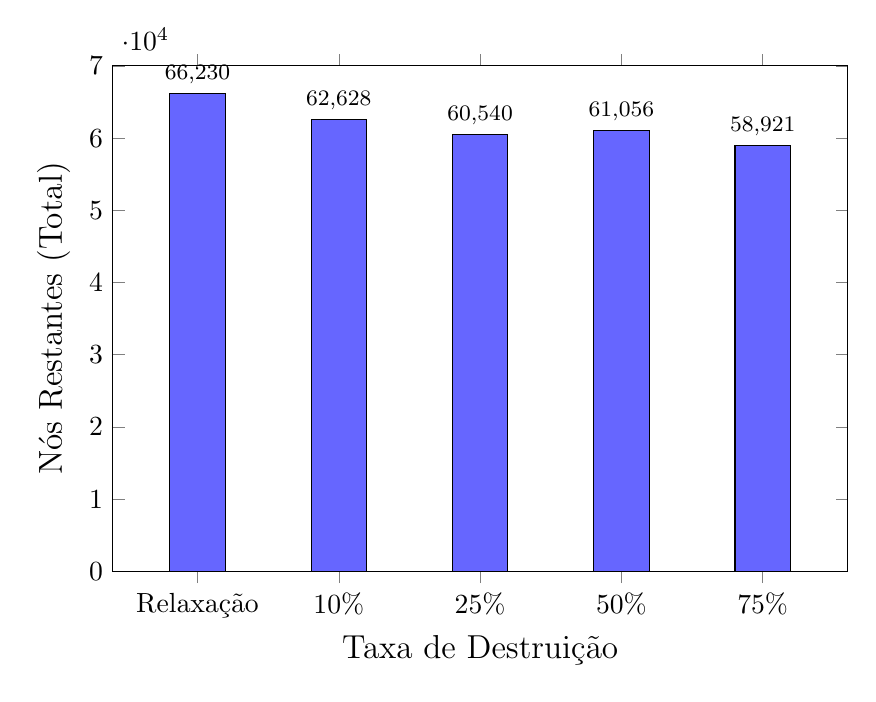
\begin{tikzpicture}
\begin{axis}[
    ybar,
    bar width=20pt,
    width=0.9\textwidth,
    height=8cm,
    ylabel={Nós Restantes (Total)},
    xlabel={Taxa de Destruição},
    symbolic x coords={Relaxação, 10\%, 25\%, 50\%, 75\%},
    xtick=data,
    nodes near coords,
    nodes near coords align={vertical},
    nodes near coords style={font=\footnotesize},
    ymin=0,
    ymax=70000,
    enlarge x limits=0.15,
    ylabel style={font=\large},
    xlabel style={font=\large},
    tick label style={font=\normalsize},
]
\addplot[fill=blue!60] coordinates {
    (Relaxação,66230)
    (10\%,62628)
    (25\%,60540)
    (50\%,61056)
    (75\%,58921)
};
\end{axis}
\end{tikzpicture}
\caption{Número total de nós restantes na árvore de Branch-and-Bound para diferentes taxas de destruição do LNS. A configuração de 75\% apresentou o melhor desempenho com 58.921 nós restantes.}
\label{fig:nodes_cand}
\end{figure}


\textbf{Gap de Otimalidade:} Em termos de gap, todas as configurações apresentaram desempenho equivalente (0,60\% total), com apenas a instância input7 permanecendo sem solução ótima. Este empate no gap reforça a importância da métrica de nodes left como critério de desempate.

\textbf{Conclusão:} A taxa de destruição de \textbf{75\%} foi selecionada para as análises subsequentes, pois demonstrou melhor capacidade de redução da árvore de busca em instâncias difíceis, indicando que vizinhanças maiores permitem ao LNS realizar explorações mais agressivas e produtivas do espaço de soluções.

\subsection{Impacto do Sentido de Ordenação (Crescente vs. Decrescente)}

Com a taxa de destruição fixada em 75\%, investigou-se o impacto do sentido de ordenação dos candidatos pelo valor de \texttt{avgPreferenceWeight}. Conforme descrito na metodologia, a ordenação crescente prioriza professores mais versáteis (maior número de preferências), enquanto a decrescente prioriza professores mais especializados (menor número de preferências).

\textbf{Resultados de Tempo:} A Tabela~\ref{tab:lns_order_tempo} revela desempenho temporal praticamente idêntico entre as duas estratégias: 180,31 segundos (crescente) versus 180,38 segundos (decrescente) no tempo médio, com diferença de apenas 0,07 segundos. Das 10 instâncias testadas, quatro atingiram o limite de tempo em ambas as configurações (input4, input15, input17 e input33), e as demais apresentaram variações inferiores a 1 segundo.

\textbf{Nodes Left:} A métrica de nós restantes revelou vantagem significativa para a ordenação crescente. A Tabela~\ref{tab:lns_order_nodes} mostra que a configuração crescente resultou em \textbf{131.997 nós restantes}, enquanto a decrescente deixou 133.674 nós, uma redução de 1.677 nós (1,25\%). Observa-se desempenho superior da ordenação crescente em duas instâncias críticas: input15 (61.546 vs. 62.452 nós) e input33 (46.243 vs. 47.063 nós). A Figura~\ref{fig:nodes_order} apresenta a comparação visual entre as três configurações.

% Gráfico: Ordenação - Nodes Left
\begin{figure}[htbp]
\centering
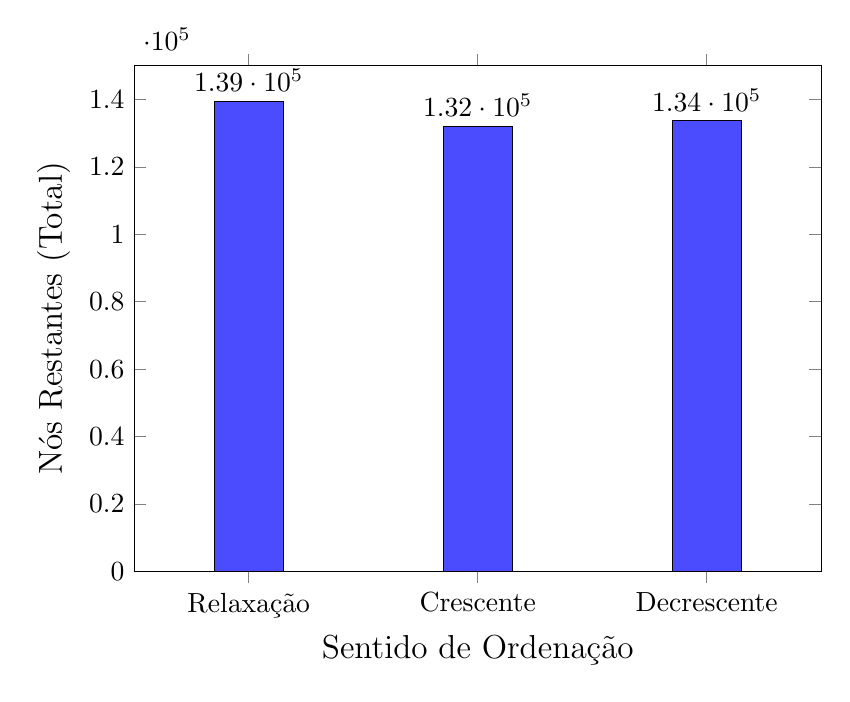
\begin{tikzpicture}
\begin{axis}[
    ybar,
    bar width=25pt,
    width=0.85\textwidth,
    height=8cm,
    ylabel={Nós Restantes (Total)},
    xlabel={Sentido de Ordenação},
    symbolic x coords={Relaxação, Crescente, Decrescente},
    xtick=data,
    nodes near coords,
    nodes near coords align={vertical},
    nodes near coords style={font=\normalsize},
    ymin=0,
    ymax=150000,
    enlarge x limits=0.25,
    ylabel style={font=\large},
    xlabel style={font=\large},
    tick label style={font=\normalsize},
]
\addplot[fill=blue!70] coordinates {
    (Relaxação,139460)
    (Crescente,131997)
    (Decrescente,133674)
};
\end{axis}
\end{tikzpicture}
\caption{Comparação do número total de nós restantes entre ordenação crescente e decrescente. A ordenação crescente (priorizando professores versáteis) obteve melhor desempenho com 131.997 nós restantes.}
\label{fig:nodes_order}
\end{figure}


\textbf{Gap de Otimalidade:} Ambas as configurações mantiveram gap total idêntico de 1,62\%, distribuído entre três instâncias não resolvidas (input4, input15 e input17), todas com gap individual de 0,20\% a 0,73\%.

\textbf{Interpretação:} A superioridade da ordenação \textbf{crescente} sugere que, para o problema DPD, priorizar a realocação de professores mais versáteis (generalistas) oferece maior flexibilidade para o sub-MIP encontrar rearranjos que melhorem a solução global. Embora professores especializados tenham menos opções de atribuição, são justamente os generalistas que permitem redistribuições mais efetivas das disciplinas, facilitando a satisfação simultânea de múltiplas restrições de carga horária.

\subsection{Impacto do Tempo Máximo do LNS (10s, 50s, 100s e 200s)}

Com os parâmetros de taxa de destruição (75\%) e ordenação (crescente) otimizados, investigou-se o impacto do limite de tempo do sub-MIP (\texttt{lns\_time}). Foram testados quatro valores: 10s, 50s, 100s e 200s, mantendo o limite global de 400 segundos por instância.

\textbf{Resultados de Tempo:} A Tabela~\ref{tab:lns_time_tempo} apresenta resultados contraintuitivos. Embora esperasse-se que limites maiores de LNS aumentassem o tempo total, observou-se comportamento não monotônico: o tempo médio foi de 164,77s (10s), 162,11s (50s), 160,27s (100s) e \textbf{159,46s (200s)}. O tempo total agregado confirma esta tendência: 1.639,76s (relaxação), 1.647,01s (10s), 1.313,60s (50s), \textbf{1.039,68s (100s)} e 1.090,00s (200s). Destaca-se a instância input15, onde as configurações de 100s e 200s resolveram o problema em $\sim$77s, contra 400s nas demais.

Esta redução de tempo com limites maiores de LNS é explicada pela capacidade de encontrar soluções de melhor qualidade mais cedo, permitindo podas mais agressivas na árvore de Branch-and-Bound. Configurações com tempo insuficiente (10s) produzem melhorias marginais que não compensam o overhead da heurística.

\textbf{Nodes Left:} A Tabela~\ref{tab:lns_time_nodes} confirma a superioridade de limites maiores. O total de nós restantes foi: 135.986 (relaxação), 144.674 (10s), 130.424 (50s), 51.935 (100s) e \textbf{33.539 (200s)}. A configuração de 200s reduziu os nós em 75,3\% em relação à relaxação pura e em 76,8\% em relação ao LNS com 10s. As instâncias input15 e input33 foram resolvidas completamente apenas com 100s ou 200s, enquanto permaneceram com dezenas de milhares de nós nas configurações inferiores. A Figura~\ref{fig:nodes_time} demonstra claramente o impacto positivo de limites maiores na redução da árvore de busca.

% Gráfico: Tempo Máximo LNS - Nodes Left
\begin{figure}[htbp]
\centering
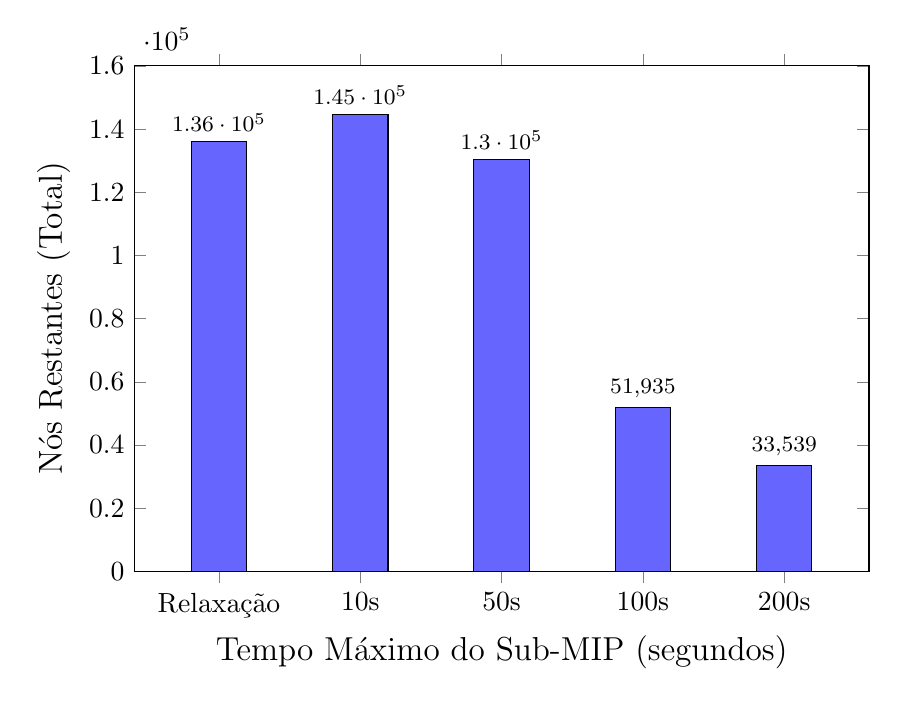
\begin{tikzpicture}
\begin{axis}[
    ybar,
    bar width=20pt,
    width=0.9\textwidth,
    height=8cm,
    ylabel={Nós Restantes (Total)},
    xlabel={Tempo Máximo do Sub-MIP (segundos)},
    symbolic x coords={Relaxação, 10s, 50s, 100s, 200s},
    xtick=data,
    nodes near coords,
    nodes near coords align={vertical},
    nodes near coords style={font=\footnotesize},
    ymin=0,
    ymax=160000,
    enlarge x limits=0.15,
    ylabel style={font=\large},
    xlabel style={font=\large},
    tick label style={font=\normalsize},
]
\addplot[fill=blue!60] coordinates {
    (Relaxação,135986)
    (10s,144674)
    (50s,130424)
    (100s,51935)
    (200s,33539)
};
\end{axis}
\end{tikzpicture}
\caption{Impacto do limite de tempo do sub-MIP no número de nós restantes. A configuração de 200s demonstrou o melhor desempenho com 33.539 nós, representando uma redução de 75,3\% em relação à relaxação pura.}
\label{fig:nodes_time}
\end{figure}


\textbf{Gap de Otimalidade:} A instância input22 manteve gap positivo em todas as configurações, mas com variação significativa nos nós restantes: 21.528 (relaxação), 29.161 (10s), 25.100 (50s), 50.411 (100s) e 33.000 (200s), sugerindo diferentes regiões de exploração.

\textbf{Conclusão:} O limite de \textbf{200 segundos} demonstrou o melhor desempenho global, reduzindo drasticamente a árvore de busca e resolvendo instâncias que outras configurações não conseguiram. O resultado evidencia que, para problemas combinatórios complexos como o DPD, investir mais tempo em cada chamada do LNS compensa através de soluções de maior qualidade que aceleram a convergência do Branch-and-Bound global. O trade-off entre intensidade (tempo por chamada) e frequência (número de chamadas) favorece claramente a intensidade para este problema.

\section{Comparativo de Desempenho e Qualidade de Solução}

\subsection{LNS versus GRASP}

\subsection{LNS versus Modelo Exato (Branch-and-Bound Padrão)}

\section{Análise de Tempo Computacional e Gap de Otimidade}